\section{Convergence Criteria for Nonsmooth DC Optimization}
\label{sec:dc-convergence-criteria}

\subsection{Criticality and $\varepsilon$-criticality}
\label{sec:finite-time-barrier}
A point $\bar\bx$ is called a \emph{critical point} of Problem~\eqref{prob:main} if
\begin{equation}
    \label{def:dc-critical}
    \zero\in \partial\phi(\bar\bx)-\partial g(\bar\bx).
\end{equation}
Equivalently, there exist $\bu\in\partial\phi(\bar\bx)$ and $\bv\in\partial g(\bar\bx)$ such that $\bu=\bv$. When both convex components are finite and locally Lipschitz around $\bar\bx$, the Clarke calculus gives $\partial_C F(\bar\bx) \subseteq \partial\phi(\bar\bx)-\partial g(\bar\bx)$. Hence, any local minimizer $\bar\bx$ of $F=\phi-g$ satisfies
\[
    \zero\in\partial_C F(\bar\bx) \subseteq \partial\phi(\bar\bx)-\partial g(\bar\bx).
\]

Exact same-point DC criticality is decomposition-dependent and may be
 weaker than Clarke stationarity of the difference function. For
example, let
\[
    \phi(x)=|x|,\qquad g(x)=|x|+x .
\]
Then \(\Psi=\phi-g=-x\), and hence
\[
    \partial_C\Psi(0)=\{-1\},
\]
so \(0\notin\partial_C\Psi(0)\). However,
\[
    \partial\phi(0)=[-1,1],\qquad \partial g(0)=[0,2],
\]
and therefore
\[
    0\in \partial\phi(0)-\partial g(0).
\]
Thus \(x=0\) is DC-critical for this particular decomposition even though
it is not Clarke-stationary for \(\Psi\). This example shows that a
finite-time lower bound for exact DC criticality cannot be obtained by
directly invoking lower bounds for pointwise Clarke stationarity of
\(\Psi\). The lower-bound construction must instead be carried out at the
level of the DC pair \((\phi,g)\) and the residual
\[
    \operatorname{dist}\bigl(0,\partial\phi(x)-\partial g(x)\bigr).
\]
% For this reason, our hard instance is built in two layers. A disjoint-kink
% background pair keeps every queried point's DC residual bounded away from
% zero, by the same resisting-oracle mechanism used at the Clarke level. A
% second, common-kink layer is then grafted onto both convex components at a
% single hidden location: it leaves the objective $F=\phi-g$, its Lipschitz
% constant, and its optimality gap completely unchanged, yet it enlarges
% $\partial\phi(x)-\partial g(x)$ at that location into a set containing
% zero, producing a point that is DC-critical without being Clarke
% stationary for $F$. This second layer is what makes the lower bound
% genuinely exercise the fact that DC criticality is weaker than Clarke
% stationarity, rather than inheriting hardness only because the two notions
% happen to coincide on the instance.

Given $\varepsilon>0$, a natural finite-time goal is the $\varepsilon$-criticality condition:
\begin{equation}
    \label{eq:exact-dc-eps-criticality}
    \operatorname{dist}\!\left( \zero, \partial\phi(\bar\bx)-\partial g(\bar\bx) \right) \le \varepsilon.
\end{equation}
This equivalently requires the existence of $\bu\in\partial\phi(\bar\bx)$ and $\bv\in\partial g(\bar\bx)$ such that $\|\bu-\bv\|\le \varepsilon$.

For comparison, the $\varepsilon$-stationarity condition for a locally Lipschitz nonsmooth nonconvex objective $F$ is $\operatorname{dist}\bigl(\zero,\partial_C F(\bar\bx)\bigr) \le \varepsilon$. Since $\partial_C F(\bar\bx) \subseteq \partial\phi(\bar\bx)-\partial g(\bar\bx)$, we have
\[
    \operatorname{dist}\!\left( \zero, \partial\phi(\bar\bx)-\partial g(\bar\bx) \right) \le \operatorname{dist}\bigl(\zero,\partial_C F(\bar\bx)\bigr).
\]
Thus, \eqref{eq:exact-dc-eps-criticality} serves as a decomposition-dependent DC analogue of Clarke $\varepsilon$-stationarity, and it ism weaker.

Zhang et al.~\citep{Zhang-2020-Complexity} established that for a broad class of Lipschitz nonsmooth nonconvex functions, no finite-time first-order algorithm can guarantee finding a point satisfying $\operatorname{dist}\bigl(\zero,\partial_C F(\bx)\bigr) \le \varepsilon$. For DC optimization, this limitation need to be re-evaluated for two reasons:
\begin{itemize}
\item[(Q1)] \emph{The DC oracle is stronger.} A DCA-type method may
query $\partial\phi$ and $\partial g$ \emph{separately}, and may even
observe $\phi(x)$ and $g(x)$ individually, whereas the obstruction of
\citet[Theorem~5]{Zhang-2020-Complexity} grants only one generalized
gradient of the whole objective. Since more information can only make
the problem easier, the lower bound is not inherited automatically.
\item[(Q2)] \emph{The DC measure is weaker.} The DC calculus gives
$\partial_C(\phi-g)(x)\subseteq\partial\phi(x)-\partial g(x)$, hence
\[
 \operatorname{dist}\bigl(0,\partial\phi(x)-\partial g(x)\bigr)
 \le
 \operatorname{dist}\bigl(0,\partial_C(\phi-g)(x)\bigr).
\]
Thus DC criticality is \emph{easier} to satisfy than Clarke
stationarity, so proving that even this weaker target is unattainable is
a strictly stronger statement than
\citet[Theorem~5]{Zhang-2020-Complexity}, not a corollary of it. A
construction whose DC residual and Clarke residual coincide everywhere
-- such as one built purely from disjoint component kinks -- proves the
Clarke-level statement but never actually tests (Q2), since the DC
target set is never larger than the Clarke target set on such an
instance. The construction below is designed so that (Q2) is tested
directly, at an explicit point where the two residuals differ.
\end{itemize}

The relevant question is whether finite-time $\varepsilon$-criticality can be achieved under this stronger DC oracle. Unfornunately, the answer is negative, as we show next. 
We settle both on a single explicit instance which is different from the hard instance constructed in \cite{Zhang-2020-Complexity}.

We formulate the lower bound under the setting where the pair $(\phi,g)$ is explicitly provided as problem data, granting the algorithm separate access to both convex components. \blue{Throughout this paper, we focus on the following subset of Lipschitz functions. For $\Delta,L,G>0$ and a fixed initial point $\bx^0$, we define:}
\[
\begin{aligned}
\mathcal D(\Delta,L,G) := \Bigl\{ (\phi,g):\;& \phi,g \text{ are proper, closed, convex, and finite-valued},\\
& F:=\phi-g \text{ is } L\text{-Lipschitz and Hadamard directionally differentiable},\\
& F(\bx^0)-\inf\limits_{\bx}F(\bx)\le \Delta,\\
& \sup\limits_{\bx} \sup\limits_{\bu\in\partial\phi(\bx),\,\bv\in\partial g(\bx)} \max\limits\{\|\bu\|,\|\bv\|\} \le G \Bigr\}.
\end{aligned}
\]
We then consider the \emph{strong} DC first-order oracle, which returns
both component values in addition to both component subgradients:
\[
    \mathcal O_{\rm DC}(\bx) = \bigl( \phi(\bx),\,g(\bx),\,\bu,\,\bv \bigr), \qquad \bu\in\partial\phi(\bx),\quad \bv\in\partial g(\bx).
\]
This dominates the weaker oracle $\bigl(F(\bx),\bu,\bv\bigr)$ used above, since $F(\bx)=\phi(\bx)-g(\bx)$ is recoverable from it; a lower bound against $\mathcal O_{\rm DC}$ is therefore the stronger statement required by (Q1). We make this claim precise as follows.
\begin{theorem}
\label{thm:dc-oracle-limitation-sketch}
Fix $\Delta,L,G>0$. There exists an absolute constant $c>0$ such that for every query budget $K\le cG/L$, every $\varepsilon\in(0,L)$, and every algorithm $\mathcal{A}$ interacting with the oracle $\mathcal O_{\rm DC}$, there exists a pair $(\phi,g)\in\mathcal D(\Delta,L,G)$ such that, with probability at least $1/2$, none of the first $K$ points $\{\bx^k\}_{k=1}^K$ queried by $\mathcal{A}$ is $\varepsilon$-critical:
\[
    \operatorname{dist}\!\left(
        \zero,\,
        \partial\phi(\bx^k)-\partial g(\bx^k)
    \right)
    >
    \varepsilon,
    \qquad k=1,\ldots,K.
\]
Moreover, the constructed pair contains a point $s$ with
\[
    \zero\in\partial\phi(s)-\partial g(s),
    \qquad
    \zero\notin\partial_C(\phi-g)(s).
\]
\end{theorem}

\begin{remark}
\label{rmk:GK-tradeoff}
Equivalently, for every $K$ the same construction gives a hard pair in $\mathcal D(\Delta,L,G_K)$ with $G_K=O(KL)$: each hidden background kink forces a slope jump in whichever convex component carries it, and monotonicity of a one-dimensional convex subgradient means these jumps accumulate rather than cancel. This $K$-dependence is specific to the one-dimensional construction; it is not present in the underlying Clarke-level obstruction of \citet{Zhang-2020-Complexity}, which does not need to keep two components separately bounded. 
% Removing the horizon restriction while keeping $G$ fixed for arbitrary $K$ would require a higher-dimensional zero-chain construction, which we leave for future work since the present statement already suffices to motivate the relaxed criticality measure introduced next.
\end{remark}
The hard instance has two layers, detailed in
\Cref{Appendix: Finite-Time Barriers of DC}.
\begin{proof}[Proof sketch]
We first construct a DC pair $(\phi_0,g_0)$ by decompositing the 
resisting-oracle construction in \citet{Zhang-2020-Complexity}.
% : given the
% $K$ queried points, it places hidden kinks between them so that every
% queried point has DC residual equal to a fixed gap $L>\varepsilon$. This
% layer is fixed once its geometric parameter is chosen; no part of it is
% hidden from the algorithm.

A common-kink layer $c_s(x)=M|x-s|+\beta-Ms$ is then added identically to
both components, $\phi_s=\phi_0+c_s$ and $g_s=g_0+c_s$. Because the same
term is added to both sides, $F=\phi_s-g_s=\phi_0-g_0$ is completely
unaffected by $s$: its Lipschitz constant, its optimality gap, and its
Clarke subdifferential everywhere are independent of $s$. Choosing the
intercept $\beta-Ms$ so that $c_s$ agrees with a fixed, $s$-independent
affine function at every point to the left of $s$ makes the entire
strong-oracle transcript -- both component values and both component
subgradients -- identical at every queried point, for every admissible
hidden location $s$ beyond the largest queried point. At $x=s$ itself,
the common kink enlarges $\partial\phi_s(s)-\partial g_s(s)$ into an
interval containing zero while leaving $\partial_C(\phi_s-g_s)(s)$
unchanged, producing the point promised in the theorem.

A two-instance argument over locations $s\neq s'$, both consistent with
the same $K$-query transcript, then shows that no algorithm can
guarantee success against both simultaneously, giving the stated
probability bound.
\end{proof}

\subsection{A Unified Notion of Approximate Criticality}
\label{sec:criticality}
In this section, we propose a unified notion to measure approximate criticality. We first recall the standard \(\delta\)-subdifferential of a proper closed convex function.

If $h:\RR^n\to\RR\cup\{+\infty\}$ is a convex function and $\delta > 0$, then for $\bar{\bx}\in\operatorname{dom} h$, the $\delta$-subdifferential of $h$ at $\bar{\bx}$ is defined by
\[
    \partial_\delta h(\bar{\bx})
    :=
    \left\{
    \bv\in\RR^n:
    h(\bz)\ge h(\bar{\bx})
    +\langle \bv,\bz-\bar{\bx}\rangle-\delta,
    \quad \forall \bz\in\RR^n
    \right\}.
\] 
When $\delta=0$, it reduces to the standard convex subdifferential. 
Figure~\ref{fig:epsilon_subgradient} illustrates that $\delta$ acts as a vertical relaxation of the supporting affine function in the geometric interpretation of the $\delta$-subgradient.

We first record the Fenchel-gap characterization of the
$\delta$-subdifferential below.
\begin{lemma}
\label{lem:fenchel-gap-toolkit}
Let $h:\RR^n\to\RR\cup\{+\infty\}$ be proper, closed, and convex, let
$\bar\bx\in\dom h$, and let $\bv\in\RR^n$, $\delta\ge0$. Then
\[
    \bv\in\partial_\delta h(\bar\bx)
    \quad\Longleftrightarrow\quad
    \Phi_h(\bar\bx,\bv)\le\delta .
\]
Moreover, $\Phi_h(\bar\bx,\bv)\ge0$ for every $\bv\in\RR^n$, and
$\bv\in\partial h(\bar\bx)$ if and only if $\Phi_h(\bar\bx,\bv)=0$.
\end{lemma}

\begin{proof}
By definition, $\bv\in\partial_\delta h(\bar\bx)$ if and only if
\begin{equation}
    h(\bz)\;\ge\;h(\bar\bx)+\langle\bv,\bz-\bar\bx\rangle-\delta
    \qquad\text{for all }\bz\in\RR^n,
    \label{eq:delta-subgrad-ineq}
\end{equation}
which, upon rearrangement, is equivalent to
\[
    \langle\bv,\bz\rangle-h(\bz)
    \;\le\;
    \langle\bv,\bar\bx\rangle-h(\bar\bx)+\delta
    \qquad\text{for all }\bz\in\RR^n.
\]
Taking the supremum over $\bz\in\RR^n$ on the left-hand side yields
$h^*(\bv)\le\langle\bv,\bar\bx\rangle-h(\bar\bx)+\delta$, that is,
$\Phi_h(\bar\bx,\bv)=h(\bar\bx)+h^*(\bv)-\langle\bv,\bar\bx\rangle
\le\delta$. Conversely, if $\Phi_h(\bar\bx,\bv)\le\delta$, then for every
$\bz\in\RR^n$,
\[
    \langle\bv,\bz\rangle-h(\bz)
    \;\le\;
    h^*(\bv)
    \;\le\;
    \langle\bv,\bar\bx\rangle-h(\bar\bx)+\delta,
\]
and rearranging recovers \eqref{eq:delta-subgrad-ineq}. The inequality
$\Phi_h(\bar\bx,\bv)\ge0$ is the Fenchel--Young inequality, and the case
$\delta=0$ gives the equality characterization of $\partial h(\bar\bx)$.
\end{proof}


\begin{figure}[t]
    \centering
    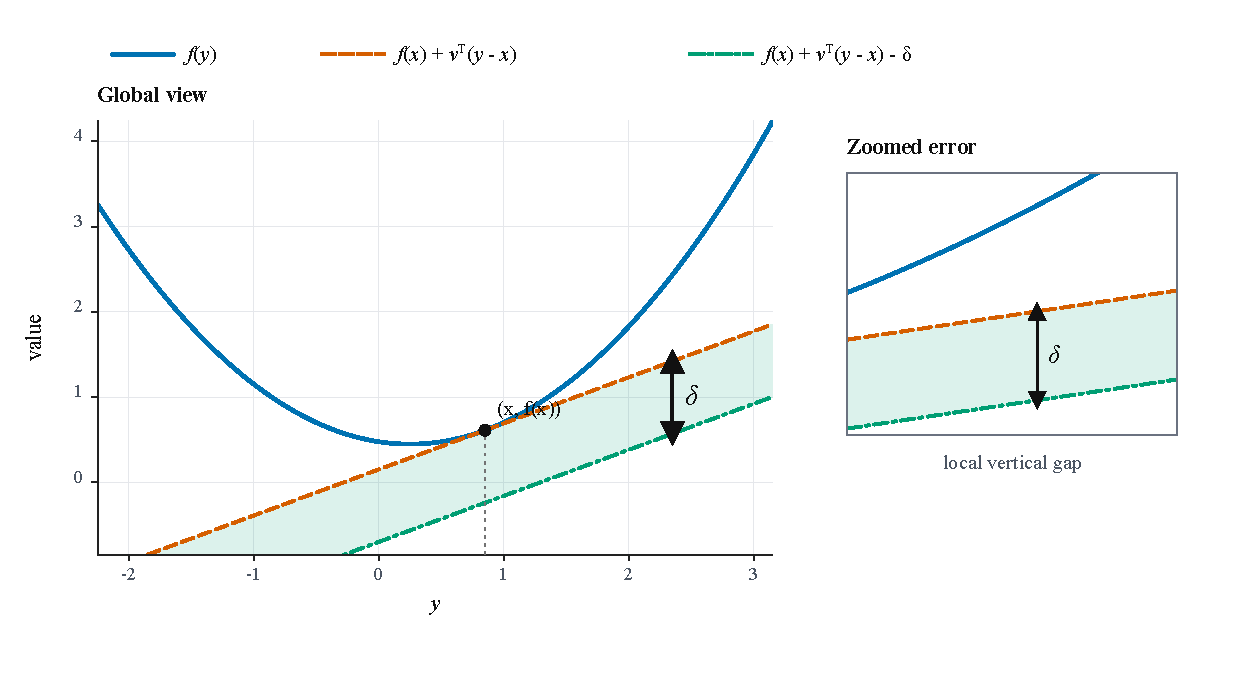
\includegraphics[width=0.7\textwidth]{epsilon_subgradient.pdf}
    \caption{Geometric interpretation of the $\delta$-subgradient. The green affine function is the ordinary supporting affine function shifted downward by $\delta$.}
    \label{fig:epsilon_subgradient}
\end{figure}

Given the limitations established in \Cref{thm:dc-oracle-limitation-sketch}, we relax the standard notion of criticality. By seeking a point in the proximity of an $\varepsilon$-critical point rather than an exact one, we are motivated to adopt the following unified definition of a $(\delta_{\phi},\delta_g,\varepsilon)$-critical point.

\begin{definition}[$(\delta_{\phi},\delta_g,\eps)$-critical point]
\label{def:delta-eps-critical}
Given \(\delta_{\phi},\delta_g\ge 0\) and \(\eps > 0\),
a point \(\bar{\bx}\in\operatorname{dom}\phi\cap\operatorname{dom}g\) is called a \((\delta_{\phi},\delta_g,\eps)\)-critical point of Problem \eqref{prob:main} if
\[
    \operatorname{dist}
    \left(
        \partial_{\delta_{\phi}}\phi(\bar{\bx}),
        \partial_{\delta_g}g(\bar{\bx})
    \right)
    \le \eps .
\]
\end{definition}


Based on this definition, we introduce the following gap functions to quantify the deviation from exact DC criticality:
\[
\begin{aligned}
    \Phi_{\phi}(\bx,\bu)
    &:=
    \phi(\bx)+\phi^*(\bu)-\langle \bu,\bx\rangle,
    \\
    \Phi_g(\bx,\bv)
    &:=
    g(\bx)+g^*(\bv)-\langle \bv,\bx\rangle.
\end{aligned}
\]

Observe that exact criticality is equivalent to the existence of a single dual vector $\bv$ such that both gap functions vanish, i.e., \(\exists \bv\) such that \(\Phi_{\phi}(\bx,\bv)=0\) and \(\Phi_g(\bx,\bv)=0\). In contrast, the $(\delta_{\phi},\delta_g,\eps)$-critical point in \Cref{def:delta-eps-critical} allows for different approximate subgradients on the two convex components, alongside a bounded mismatch between these dual vectors:
\[
\begin{aligned}
    \exists \bu,\bv,\qquad
    \Phi_{\phi}(\bx,\bu)\le \delta_{\phi},\quad
    \Phi_g(\bx,\bv)\le \delta_g, \quad 
    \|\bu-\bv\|\le \eps .
\end{aligned}
\]

When $\delta_{\phi}=\delta_g=0$, the $(0,0,\eps)$-critical point reduces to the classical $\varepsilon$-critical point. In fact, the $(\delta_{\phi},\delta_g,\eps)$-criticality serves as a more reliable diagnostic metric for approximate criticality. For nonsmooth DC functions, classical point-based stationarity residuals can remain stubbornly large ($\mathcal{O}(1)$) near a nonsmooth minimizer, whereas our proposed Fenchel-gap metric smoothly converges to zero. The following one-dimensional, closed-form example makes this diagnostic obstruction explicit.

\begin{figure}[t]
\centering
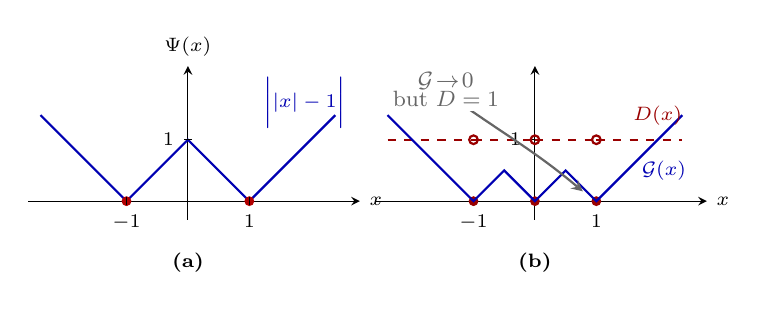
\begin{tikzpicture}[>=stealth, font=\scriptsize, scale=0.78]
 
% ================================================================
% Panel (a):  Psi(x) = ||x|-1|
% ================================================================
\begin{scope}[xshift=0cm]
 
  % axes
  \draw[->] (-2.6,0) -- (2.8,0) node[right] {$x$};
  \draw[->] (0,-0.3) -- (0,2.2) node[above] {$\Psi(x)$};
 
  % Psi(x) = ||x|-1|
  % key points: (-2,1) (-1,0) (0,1) (1,0) (2,1)
  \draw[thick, blue!70!black]
    (-2.4,1.4) -- (-1,0) -- (0,1) -- (1,0) -- (2.4,1.4);
 
  % mark minimizers
  \filldraw[red!70!black] (-1,0) circle (2pt);
  \filldraw[red!70!black] ( 1,0) circle (2pt);
 
  % tick marks
  \draw (-1,0.07) -- (-1,-0.07) node[below] {$-1$};
  \draw ( 1,0.07) -- ( 1,-0.07) node[below] {$1$};
  \draw (0.07,1) -- (-0.07,1) node[left] {$1$};
 
  % label
  \node[blue!70!black] at (1.9,1.6) {$\bigl||x|-1\bigr|$};
 
  % panel label
  \node at (0,-1.0) {\textbf{(a)}};
 
\end{scope}
 
% ================================================================
% Panel (b):  D(x) vs G(x)
% ================================================================
\begin{scope}[xshift=5.65cm]
 
  % axes
  \draw[->] (-2.6,0) -- (2.8,0) node[right] {$x$};
  \draw[->] (0,-0.3) -- (0,2.2);
 
  % tick marks
  \draw (-1,0.07) -- (-1,-0.07) node[below] {$-1$};
  \draw ( 1,0.07) -- ( 1,-0.07) node[below] {$1$};
  \draw (0.07,1) -- (-0.07,1) node[left] {$1$};
 
  % --- D(x): dashed, step function at 1, with jumps at {-1,0,1} ---
  \draw[thick, dashed, red!60!black]
    (-2.4,1) -- (-1,1);
  \draw[thick, dashed, red!60!black]
    (-1,1) -- (0,1);
  \draw[thick, dashed, red!60!black]
    (0,1) -- (1,1);
  \draw[thick, dashed, red!60!black]
    (1,1) -- (2.4,1);
 
  % open circles at D=1 for x in {-1,0,1}
  \draw[red!60!black, thick] (-1,1) circle (2pt);
  \draw[red!60!black, thick] ( 0,1) circle (2pt);
  \draw[red!60!black, thick] ( 1,1) circle (2pt);
 
  % closed circles at D=0 for x in {-1,0,1}
  \filldraw[red!60!black] (-1,0) circle (2pt);
  \filldraw[red!60!black] ( 0,0) circle (2pt);
  \filldraw[red!60!black] ( 1,0) circle (2pt);
 
  % --- G(x): solid, piecewise linear ---
  % G(x) = |x|              for 0<=|x|<=1/2
  %       = 1-|x|           for 1/2<=|x|<=1
  %       = |x|-1           for |x|>=1
  % key points: (-2,1) (-1,0) (-0.5,0.5) (0,0) (0.5,0.5) (1,0) (2,1)
  \draw[thick, blue!70!black]
    (-2.4,1.4) -- (-1,0) -- (-0.5,0.5) -- (0,0)
    -- (0.5,0.5) -- (1,0) -- (2.4,1.4);
 
  % labels
  \node[red!60!black]  at (2.0, 1.4) {$D(x)$};
  \node[blue!70!black] at (2.1, 0.5) {$\mathcal{G}(x)$};
 
  % annotation arrow: highlight the gap near x=1
  \draw[->, thick, black!60] (-1.25,1.62) to[out=-35,in=140] (0.78,0.16);
  \node[black!60, align=center, fill=white, inner sep=1.5pt]
    at (-1.45,1.82)
    {\footnotesize $\mathcal{G}\!\to\!0$\\[-1pt]\footnotesize but $D=1$};
 
  % panel label
  \node at (0,-1.0) {\textbf{(b)}};
 
\end{scope}
\end{tikzpicture}
\caption{Exact critical-distance residual versus Fenchel-gap behavior in the one-dimensional example.}
\label{fig:exact-vs-fenchel-gap}
\end{figure}

\begin{example}[Exact vs.\ Fenchel-gap certificate]
\label{ex:motivating-dc-gap}
Consider
\[
    \Psi(x)=\bigl||x|-1\bigr|
    =
    \phi(x)-g(x),
\]
where \( \phi(x)=3+4(|x|-1)_+ \) and \( g(x)=|x+1|+|x|+|x-1| \). Both \(\phi\) and \(g\) are convex, and \(g\) is nonsmooth at the global minimizers \(x=\pm1\). The exact same-point critical-distance residual is
\[
    D(x)
    :=
    \operatorname{dist}\bigl(0,\partial\phi(x)-\partial g(x)\bigr)
    =
    \begin{cases}
    0, & x\in\{-1,0,1\},\\
    1, & \text{otherwise}.
    \end{cases}
\]
Hence, even when \(x\) is arbitrarily close to the nonsmooth minimizer \(x=1\), the exact critical distance remains \(D(x)=1\).

For comparison, specialize the two-sided Fenchel certificate to the common-certificate scalar gap
\[
    \calG(x)
    :=
    \inf\limits_{b\in\RR}
    \left\{
        \Phi_\phi(x,b)+\Phi_g(x,b)
    \right\}.
\]
This corresponds to the case \(\bu=\bv=b\): the same scalar \(b\) must act as an approximate subgradient certificate for both convex components at the same point. A direct conjugate calculation gives
\[
\begin{aligned}
    \phi^*(b)
    &=
    \begin{cases}
        |b|-3, & |b|\le 4,\\
        +\infty, & |b|>4,
    \end{cases}
    \\
    g^*(b)
    &=
    \begin{cases}
        -2, & |b|\le 1,\\
        |b|-3, & 1\le |b|\le 3,\\
        +\infty, & |b|>3.
    \end{cases}
\end{aligned}
\]
Consequently,
\[
    \calG(x)
    =
    \begin{cases}
        |x|, & 0\le |x|\le \frac12,\\
        1-|x|, & \frac12\le |x|\le 1,\\
        |x|-1, & |x|\ge 1.
    \end{cases}
\]
In particular, \(\calG(x)\to0\) as \(x\to\pm1\), while \(D(x)=1\) for every \(x\notin\{-1,0,1\}\). Equivalently, near \(x=1\), choosing \(b=1\in\partial g(x)\) for \(0<x<1\) gives
\[
    \Phi_g(x,1)=0,
    \qquad
    \Phi_\phi(x,1)=1-x\to0
    \;\;\text{as }x\uparrow1,
\]
and choosing \(b=3\in\partial g(x)\) for \(x>1\) gives
\[
    \Phi_g(x,3)=0,
    \qquad
    \Phi_\phi(x,3)=x-1\to0
    \;\;\text{as }x\downarrow1.
\]
This is the behavior shown in \Cref{fig:exact-vs-fenchel-gap}: the Fenchel gap accurately detects convergence toward a nonsmooth minimizer, whereas the exact critical distance remains an \(O(1)\) step function around it.
\end{example}

\Cref{ex:motivating-dc-gap} shows that the $(\delta_\phi,\delta_g,\varepsilon)$-critical point repairs the diagnostic failure of the exact residual, but a diagnostic that is easy to satisfy is only useful if it is also sound: an overly permissive relaxation could remain satisfiable at points bearing no relation to criticality at all. We close this section by ruling out this concern as follows.
 The next proposition shows that \Cref{def:delta-eps-critical} degenerates correctly, in the sense that driving all three tolerances to zero forces exact DC criticality at the same point.
This properpsition depends on the monotonicity of the $\delta$-subdifferential in $\delta$ together with lower semicontinuity of $\phi,\phi^*,g,g^*$; 

\begin{proposition}
\label{prop:exact-consistency}
Suppose $\phi$ and $g$ are $G$-Lipschitz on $\RR^n$. If $\bar\bx$ is a $(\delta_\phi^{(k)},\delta_g^{(k)},\varepsilon^{(k)})$-critical point of Problem~\eqref{prob:main} for every $k\in\NN$, with $\delta_\phi^{(k)},\delta_g^{(k)},\varepsilon^{(k)}\to0$ as $k\to\infty$, then $\bar\bx$ is a critical point of Problem~\eqref{prob:main}, i.e., $\zero\in\partial\phi(\bar\bx)-\partial g(\bar\bx)$.
\end{proposition}

\begin{proof}
For each $k$, choose $\bu_k\in\partial_{\delta_\phi^{(k)}}\phi(\bar\bx)$ and $\bv_k\in\partial_{\delta_g^{(k)}}g(\bar\bx)$ with $\|\bu_k-\bv_k\|\le\varepsilon^{(k)}$. Since $\phi$ is $G$-Lipschitz on all of $\RR^n$, every element of $\partial_\delta\phi(\bar\bx)$ has norm at most $G$, regardless of $\delta$: for $\bv\in\partial_\delta\phi(\bar\bx)$, the defining inequality $\phi(\bar\bx)+G\|\bz-\bar\bx\|\ge\phi(\bz)\ge\phi(\bar\bx)+\langle\bv,\bz-\bar\bx\rangle-\delta$ along $\bz-\bar\bx=t\bv/\|\bv\|$ forces $\|\bv\|\le G+\delta/t$ for every $t>0$, hence $\|\bv\|\le G$ as $t\to\infty$. The same bound holds for $\partial_\delta g(\bar\bx)$. Thus $\{\bu_k\}$ and $\{\bv_k\}$ are bounded, and we may pass to a subsequence along which $\bu_k\to\bu^\star$ and $\bv_k\to\bv^\star$; since $\|\bu_k-\bv_k\|\to0$, we get $\bu^\star=\bv^\star=:\bw$.

It remains to show $\bw\in\partial\phi(\bar\bx)$; the argument for $\bw\in\partial g(\bar\bx)$ is identical. Since $\phi$ and $\phi^*$ are proper, closed, and convex, both are lower semicontinuous, so
\[
    \Phi_\phi(\bar\bx,\bw)
    =\phi(\bar\bx)+\phi^*(\bw)-\langle\bw,\bar\bx\rangle
    \le\liminf_{k\to\infty}\Bigl[\phi(\bar\bx)+\phi^*(\bu_k)-\langle\bu_k,\bar\bx\rangle\Bigr]
    =\liminf_{k\to\infty}\Phi_\phi(\bar\bx,\bu_k)
    \le\liminf_{k\to\infty}\delta_\phi^{(k)}=0.
\]
The Fenchel--Young inequality gives $\Phi_\phi(\bar\bx,\bw)\ge0$ unconditionally, so $\Phi_\phi(\bar\bx,\bw)=0$, i.e., $\bw\in\partial\phi(\bar\bx)$. Hence $\bw\in\partial\phi(\bar\bx)\cap\partial g(\bar\bx)$, and $\zero=\bw-\bw\in\partial\phi(\bar\bx)-\partial g(\bar\bx)$.
\end{proof}


% no spatial displacement argument is needed, since the collapse takes place at the fixed point $\bar\bx$. This is a first indication of a recurring theme in \Cref{sec:relationship-relaxed-dc-criticality} below: relaxing criticality along the value axis, rather than the spatial axis, tends to keep the base point fixed throughout.

\subsection{Relationship between Relaxed DC Criticality Notions}
\label{sec:relationship-relaxed-dc-criticality}

We show that the $(\delta_\phi,\delta_g,\varepsilon)$-critical point in
\Cref{def:delta-eps-critical} is a unifying value-relaxed formulation:
every previously proposed relaxed DC criticality notion for
Problem~\eqref{prob:main} embeds into
\Cref{def:delta-eps-critical} for a suitable choice of
$(\delta_\phi,\delta_g,\varepsilon)$, and this embedding admits a sharper,
second-order accurate rate whenever the underlying component is smooth.

We recall three such notions, in increasing order of the spatial freedom
they allow.

\begin{definition}[$\varepsilon$-critical point~\citep{moudafi2021complete,sun2023algorithms}]
\label{Def: epsilon-critical point in DC}
Given $\varepsilon>0$, a point $\bar\bx\in\RR^n$ is an $\varepsilon$-critical
point of Problem~\eqref{prob:main} if there exist
$\bar\by\in\RR^n$ and $\bar\bu\in\partial\phi(\bar\bx)-\partial g(\bar\by)$
such that
\[
    \max\limits\{\|\bar\bu\|,\|\bar\bx-\bar\by\|\}\le\varepsilon .
\]
\end{definition}

\begin{definition}[Nearly $\varepsilon$-critical point~\citep{yao2022large}]
\label{Def: epsilon-critical point 3}
Given $\varepsilon>0$, a point $\bar\bx\in\RR^n$ is a nearly
$\varepsilon$-critical point of Problem~\eqref{prob:main}
if there exist $\bar\by_1,\bar\by_2\in\RR^n$ and
$\bar\bu\in\partial\phi(\bar\by_1)-\partial g(\bar\by_2)$ such that
\[
    \max\limits\{\|\bar\bu\|,\|\bar\bx-\bar\by_1\|,\|\bar\bx-\bar\by_2\|\}
    \le\varepsilon .
\]
\end{definition}

\begin{definition}[Nearly $\varepsilon$-stationary point~\citep{xu2019stochastic}]
\label{def:xu-near-stationary}
Given $\varepsilon>0$, a point $\bar\bx\in\RR^n$ is a nearly
$\varepsilon$-stationary point of Problem~\eqref{prob:main} if there exist
$c>0$ and $\bx^*\in\RR^n$ with
$\|\bar\bx-\bx^*\|\le c\varepsilon$ such that
\[
    \operatorname{dist}\bigl(\partial\phi(\bx^*),\partial g(\bx^*)\bigr)
    \le\varepsilon .
\]
\end{definition}

Definitions~\ref{Def: epsilon-critical point in DC} and
\ref{Def: epsilon-critical point 3} relax criticality by letting $\phi$
and $g$ be evaluated at points that may drift apart from each other and
from $\bar\bx$; \Cref{def:xu-near-stationary} instead forces $\phi$ and
$g$ to share a common witness point $\bx^*$, which itself may drift from
$\bar\bx$. All three reduce to a single mechanism: converting a spatial
offset into a Fenchel-gap slack.

\begin{lemma}
\label{lem:spatial-to-value}
Let $q:\RR^n\to\RR\cup\{+\infty\}$ be proper, closed, convex, and
$G$-Lipschitz on a convex set containing $\bx,\by\in\operatorname{dom}q$.
\begin{enumerate}
    \item[(a)] If $\bv\in\partial q(\by)$, then
    $\bv\in\partial_{2G\|\bx-\by\|}q(\bx)$.
    \item[(b)] If, in addition, $q$ is $L$-smooth on this set and
    $\bv=\nabla q(\by)$, then
    $\bv\in\partial_{\frac{L}{2}\|\bx-\by\|^2}q(\bx)$.
\end{enumerate}
\end{lemma}

\begin{proof}
By the Fenchel--Young equality at a subgradient,
$q^*(\bv)=\langle\bv,\by\rangle-q(\by)$, so
\[
    \Phi_q(\bx,\bv)
    = q(\bx)-q(\by)-\langle\bv,\bx-\by\rangle
    =: D_q(\bx,\by).
\]
(a) Convexity gives $D_q(\bx,\by)\ge0$; $G$-Lipschitzness gives
$q(\bx)-q(\by)\le G\|\bx-\by\|$ and $\|\bv\|\le G$, so
$D_q(\bx,\by)\le 2G\|\bx-\by\|$.
(b) $D_q(\bx,\by)$ is the Bregman divergence of $q$ at $(\bx,\by)$; for
convex $L$-smooth $q$ it satisfies $0\le D_q(\bx,\by)\le\tfrac
L2\|\bx-\by\|^2$ by the descent lemma.
\end{proof}
We then establish that the $(\delta_\phi,\delta_g,\varepsilon)$-critical point in \Cref{def:delta-eps-critical} recovers all three existing relaxed DC criticality notions
\begin{proposition}
\label{prop:recovery-existing-dc-criticality}
Suppose $\phi$ and $g$ are, respectively, $G_\phi$- and $G_g$-Lipschitz on
the relevant neighborhoods below. Then:
\begin{enumerate}
    \item[(i)] If $\bar\bx$ is an $\varepsilon$-critical point in the
    sense of \Cref{Def: epsilon-critical point in DC}, then $\bar\bx$ is a
    $(0,\,2G_g\varepsilon,\,\varepsilon)$-critical point.
    \item[(ii)] If $\bar\bx$ is a nearly $\varepsilon$-critical point in
    the sense of \Cref{Def: epsilon-critical point 3}, then $\bar\bx$ is a
    $(2G_\phi\varepsilon,\,2G_g\varepsilon,\,\varepsilon)$-critical point.
    \item[(iii)] If $\bar\bx$ is a nearly $\varepsilon$-stationary point in
    the sense of \Cref{def:xu-near-stationary}, then $\bar\bx$ is a
    $(2G_\phi c\varepsilon,\,2G_g c\varepsilon,\,\varepsilon)$-critical
    point.
\end{enumerate}
\end{proposition}

\begin{proof}
(i) Write $\bar\bu=\bp-\bq$ with $\bp\in\partial\phi(\bar\bx)
=\partial_0\phi(\bar\bx)$ and $\bq\in\partial g(\bar\by)$.
\Cref{lem:spatial-to-value}(a) with $q=g$, $\bx=\bar\bx$, $\by=\bar\by$
gives $\bq\in\partial_{2G_g\|\bar\bx-\bar\by\|}g(\bar\bx)\subseteq
\partial_{2G_g\varepsilon}g(\bar\bx)$, so
$\operatorname{dist}(\partial_0\phi(\bar\bx),\partial_{2G_g\varepsilon}g(\bar\bx))
\le\|\bp-\bq\|=\|\bar\bu\|\le\varepsilon$.

(ii) Identical, applying \Cref{lem:spatial-to-value}(a) to both
$\bp\in\partial\phi(\bar\by_1)$ and $\bq\in\partial g(\bar\by_2)$.

(iii) Take $\bp\in\partial\phi(\bx^*)$, $\bq\in\partial g(\bx^*)$ with
$\|\bp-\bq\|\le\varepsilon$; this is exactly case (ii) with
$\bar\by_1=\bar\by_2=\bx^*$ and spatial offset $c\varepsilon$ in place of
$\varepsilon$.
\end{proof}

\begin{remark}
Case (iii) is not an independent construction: it is case (ii)
specialized to a common witness point. The distinction between
\Cref{Def: epsilon-critical point in DC}/\ref{Def: epsilon-critical point 3}
and \Cref{def:xu-near-stationary} is therefore not a difference in the
relaxation mechanism, but only in whether the two witness points are
allowed to coincide.
\end{remark}

The embedding above only uses Lipschitz continuity and is tight up to
constants. When a component happens to be smooth,
\Cref{lem:spatial-to-value}(b) applies in place of (a) and yields a
second-order accurate slack on that side.

\begin{proposition}
\label{prop:sharp-smooth}
In the setting of \Cref{def:xu-near-stationary}, suppose in addition that
$g$ is convex and $L_g$-smooth on a neighborhood of $\bx^*$. Then
$\bar\bx$ is a
\[
    \Bigl(2G_\phi c\varepsilon,\ \tfrac{L_g}{2}c^2\varepsilon^2,\
    \varepsilon\Bigr)\text{-critical point}.
\]
If $\phi$ is also convex and $L_\phi$-smooth on a neighborhood of
$\bx^*$, the first slack sharpens to $\tfrac{L_\phi}{2}c^2\varepsilon^2$,
so that $\bar\bx$ is an
$\bigl(\mathcal O(\varepsilon^2),\,\mathcal O(\varepsilon^2),\,
\varepsilon\bigr)$-critical point.
\end{proposition}

\begin{proof}
Take $\bv^*=\nabla g(\bx^*)$ in place of an arbitrary
$\bq\in\partial g(\bx^*)$ in the proof of
\Cref{prop:recovery-existing-dc-criticality}(iii), and apply
\Cref{lem:spatial-to-value}(b) instead of (a):
$\bv^*\in\partial_{\frac{L_g}{2}\|\bar\bx-\bx^*\|^2}g(\bar\bx)
\subseteq\partial_{\frac{L_g}{2}c^2\varepsilon^2}g(\bar\bx)$. The
$\phi$-side bound is unchanged from
\Cref{prop:recovery-existing-dc-criticality}(iii). The refinement when
$\phi$ is also smooth follows by the same substitution on the
$\phi$-side.
\end{proof}

\Cref{prop:recovery-existing-dc-criticality} and
\Cref{prop:sharp-smooth} together show that
\Cref{def:delta-eps-critical} strictly subsumes
Definitions~\ref{Def: epsilon-critical point in DC},
\ref{Def: epsilon-critical point 3}, and \ref{def:xu-near-stationary}: the
value slack incurred is $\mathcal O(\varepsilon)$ under Lipschitz
continuity alone, and tightens to $\mathcal O(\varepsilon^2)$ on any
component that is additionally smooth. This also isolates precisely what
smoothness of $g$ buys in \citet{xu2019stochastic}: it is not needed for
the embedding into \Cref{def:delta-eps-critical}, which only requires
Lipschitz continuity, but it tightens the resulting slack by one order in
$\varepsilon$.

\subsubsection{The Converse Embedding}

\Cref{prop:recovery-existing-dc-criticality} and \Cref{prop:sharp-smooth}
show that $(\delta_\phi,\delta_g,\varepsilon)$-criticality is no harder to
satisfy than any previously proposed relaxed DC criticality notion. We now
establish the converse direction: satisfying \Cref{def:delta-eps-critical}
is also no easier, in the sense that it forces the same qualitative
conclusion as \Cref{Def: epsilon-critical point 3}, up to an explicit loss
of one order in the tolerance. The mechanism is the classical reachback
theorem of Brøndsted and Rockafellar~\citep{brondsted1965subdifferentiability},
which converts an approximate subgradient at $\bar\bx$ into an exact
subgradient at a nearby point, and is the exact converse of
\Cref{lem:spatial-to-value}(a).

\begin{lemma}
\label{lem:value-to-spatial}
Let $q:\RR^n\to\RR\cup\{+\infty\}$ be proper, closed, and convex, and let
$\bv\in\partial_\delta q(\bar\bx)$ for some $\delta>0$. Then for every
$\lambda>0$ there exist $\hat\bx\in\RR^n$ and $\hat\bv\in\partial
q(\hat\bx)$ such that
\[
    \|\hat\bx-\bar\bx\|\le\lambda,
    \qquad
    \|\hat\bv-\bv\|\le\frac{\delta}{\lambda}.
\]
In particular, taking $\lambda=\sqrt\delta$ gives
$\|\hat\bx-\bar\bx\|\le\sqrt\delta$ and $\|\hat\bv-\bv\|\le\sqrt\delta$.
\end{lemma}

\begin{proposition}[Reverse embedding]
\label{prop:reverse-embedding}
If $\bar\bx$ is a $(\delta_\phi,\delta_g,\varepsilon)$-critical point of
Problem~\eqref{prob:main}, then $\bar\bx$ is a nearly
$\varepsilon'$-critical point in the sense of
\Cref{Def: epsilon-critical point 3}, with
\[
    \varepsilon'=\varepsilon+\sqrt{\delta_\phi}+\sqrt{\delta_g}.
\]
\end{proposition}

\begin{proof}
Let $\bu\in\partial_{\delta_\phi}\phi(\bar\bx)$ and
$\bv\in\partial_{\delta_g}g(\bar\bx)$ with $\|\bu-\bv\|\le\varepsilon$.
Apply \Cref{lem:value-to-spatial} to $\bu$ with $\lambda=\sqrt{\delta_\phi}$
and to $\bv$ with $\lambda=\sqrt{\delta_g}$, obtaining $\bar\by_1$,
$\hat\bu\in\partial\phi(\bar\by_1)$ and $\bar\by_2$,
$\hat\bv\in\partial g(\bar\by_2)$ with $\|\bar\by_1-\bar\bx\|\le\sqrt{\delta_\phi}$,
$\|\hat\bu-\bu\|\le\sqrt{\delta_\phi}$, and analogously for
$\bar\by_2,\hat\bv$. Set $\bar\bu:=\hat\bu-\hat\bv\in\partial\phi(\bar\by_1)-\partial g(\bar\by_2)$. The triangle inequality gives
\[
    \|\bar\bu\|
    \le\|\hat\bu-\bu\|+\|\bu-\bv\|+\|\bv-\hat\bv\|
    \le\sqrt{\delta_\phi}+\varepsilon+\sqrt{\delta_g}=\varepsilon',
\]
while $\|\bar\bx-\bar\by_1\|\le\sqrt{\delta_\phi}\le\varepsilon'$ and
$\|\bar\bx-\bar\by_2\|\le\sqrt{\delta_g}\le\varepsilon'$, which verifies the
defining condition of \Cref{Def: epsilon-critical point 3} with
$\varepsilon'$ in place of $\varepsilon$.
\end{proof}

\begin{proposition}[Same-point refinement under smoothness]
\label{prop:reverse-smooth}
In the setting of \Cref{prop:reverse-embedding}, suppose in addition that
$g$ is convex and $L_g$-smooth on a neighborhood of $\bar\bx$. Then
\[
    \operatorname{dist}\bigl(\nabla g(\bar\bx),\,\partial_{\delta_\phi}\phi(\bar\bx)\bigr)
    \le\varepsilon+\sqrt{2L_g\delta_g}.
\]
If $\phi$ is also convex and $L_\phi$-smooth on a neighborhood of
$\bar\bx$, then
\[
    \bigl\|\nabla\phi(\bar\bx)-\nabla g(\bar\bx)\bigr\|
    \le\varepsilon+\sqrt{2L_\phi\delta_\phi}+\sqrt{2L_g\delta_g},
\]
so that $\bar\bx$ is, up to this explicit slack, a same-point approximate
stationary point of the smooth DC problem.
\end{proposition}

\begin{proof}
For $L_g$-smooth convex $g$, the conjugate $g^*$ is
$\tfrac1{L_g}$-strongly convex, so $\Phi_g(\bar\bx,\bv)\ge
\tfrac1{2L_g}\|\bv-\nabla g(\bar\bx)\|^2$ for every $\bv$. Applied to
$\bv\in\partial_{\delta_g}g(\bar\bx)$, this gives
$\|\bv-\nabla g(\bar\bx)\|\le\sqrt{2L_g\delta_g}$; combined with
$\bu\in\partial_{\delta_\phi}\phi(\bar\bx)$ and $\|\bu-\bv\|\le\varepsilon$,
the triangle inequality gives the first bound. The second bound follows by
the same argument applied to $\bu$ once $\phi$ is also $L_\phi$-smooth and
convex.
\end{proof}

\begin{remark}[Asymmetry between the two directions]
The two directions are not symmetric. Embedding an existing notion into
\Cref{def:delta-eps-critical} costs a value slack linear in the spatial
tolerance under Lipschitz continuity alone (\Cref{lem:spatial-to-value}(a))
and quadratic under smoothness (\Cref{lem:spatial-to-value}(b)). Recovering
an existing notion from \Cref{def:delta-eps-critical} costs a spatial
displacement on the order of the square root of the value tolerance under
Lipschitz continuity alone (\Cref{lem:value-to-spatial}); this square-root
rate is the classical Brøndsted--Rockafellar rate and is not, in general,
improvable to a linear one. Smoothness removes the asymmetry in the
strongest sense: on a smooth component, the reverse direction also
collapses to a same-point bound (\Cref{prop:reverse-smooth}), matching the
same-point character of the forward direction under smoothness
(\Cref{prop:sharp-smooth}), at the cost of a square-root rather than a
quadratic rate.
\end{remark}

\subsubsection{Relation to Goldstein Stationarity}

We conclude by relating $(\delta_\phi,\delta_g,\varepsilon)$-criticality to
a relaxed stationarity notion outside the DC literature: the Goldstein
$\delta$-subdifferential relaxation of Clarke stationarity
\citep{goldstein1977optimization,Zhang-2020-Complexity}, introduced
schematically in \Cref{fig:goldstein-vs-approximate-subdifferential}. For a
locally Lipschitz function $F:\RR^n\to\RR$, the Goldstein
$\delta$-subdifferential at $\bar\bx$ is
\[
    \partial_\delta^G F(\bar\bx)
    :=
    \overline{\operatorname{conv}}
    \bigcup_{\by\in B_\delta(\bar\bx)}
    \partial_C F(\by),
\]
and $\bar\bx$ is a $(\delta,\varepsilon)$-Goldstein stationary point of $F$
if $\operatorname{dist}(\zero,\partial_\delta^G F(\bar\bx))\le\varepsilon$,
where $B_\delta(\bar\bx):=\{\by\in\RR^n:\|\by-\bar\bx\|\le\delta\}$.
Applied to $F=\Psi=\phi-g$, this relaxes Clarke stationarity along the
spatial axis: it collects exact generalized gradients over a
$\delta$-neighborhood of $\bar\bx$ and convexifies, rather than relaxing
the defining inequality at $\bar\bx$ itself. \Cref{def:delta-eps-critical}
relaxes along the orthogonal, value axis, and couples $\phi$ and $g$
independently rather than through a common witness point in
$B_\delta(\bar\bx)$. \Cref{tab:goldstein-vs-ours} summarizes the
distinction.

\begin{table}[t]
\centering
\caption{Two relaxation mechanisms for the same base criterion
$\zero\in\partial\phi(\bar\bx)-\partial g(\bar\bx)$.}
\label{tab:goldstein-vs-ours}
\small
\begin{tabular}{lll}
\hline
 & $(\delta,\varepsilon)$-Goldstein & $(\delta_\phi,\delta_g,\varepsilon)$-critical \\
\hline
Relaxation axis & spatial, $B_\delta(\bar\bx)$ & value, Fenchel--Young gap \\
Witness structure & common $\by\in B_\delta(\bar\bx)$ & independent $\bu,\bv$ at $\bar\bx$ \\
Evaluation point & nearby $\by$ & $\bar\bx$ itself \\
\hline
\end{tabular}
\end{table}

Despite this structural difference, the Goldstein relaxation embeds into
ours.

\begin{lemma}[Goldstein bridge]
\label{cor:goldstein-bridge}
Let $q:\RR^n\to\RR\cup\{+\infty\}$ be proper, closed, convex, and
$G$-Lipschitz on a convex set containing $B_\delta(\bar\bx)$. Then
\[
    \bigcup_{\by\in B_\delta(\bar\bx)}\partial q(\by)
    \subseteq
    \partial_{2G\delta}q(\bar\bx).
\]
\end{lemma}

\begin{proof}
Immediate from \Cref{lem:spatial-to-value}(a): for $\by\in B_\delta(\bar\bx)$
and $\bv\in\partial q(\by)$, $\|\bar\bx-\by\|\le\delta$ gives
$\bv\in\partial_{2G\delta}q(\bar\bx)$.
\end{proof}

\begin{proposition}[Goldstein implies ours]
\label{prop:goldstein-implies-ours}
Suppose $\phi,g$ are, respectively, $G_\phi$- and $G_g$-Lipschitz on a
convex set containing $B_\delta(\bar\bx)$. If $\bar\bx$ is a
$(\delta,\varepsilon)$-Goldstein stationary point of $\Psi=\phi-g$, then
$\bar\bx$ is a $(2G_\phi\delta,\,2G_g\delta,\,\varepsilon)$-critical point.
\end{proposition}

\begin{proof}
Let $\bw\in\partial_\delta^G\Psi(\bar\bx)$ with $\|\bw\|\le\varepsilon$. By
Carath\'eodory's theorem, $\bw=\sum_i\lambda_i\bw_i$ for finitely many
$\bw_i\in\partial_C\Psi(\by_i)$, $\by_i\in B_\delta(\bar\bx)$,
$\lambda_i\ge0$, $\sum_i\lambda_i=1$. By the Clarke sum rule for the
difference of two convex functions, $\bw_i=\bu_i-\bv_i$ with
$\bu_i\in\partial\phi(\by_i)$, $\bv_i\in\partial g(\by_i)$. Set
$\bar\bu:=\sum_i\lambda_i\bu_i$ and $\bar\bv:=\sum_i\lambda_i\bv_i$. By
\Cref{cor:goldstein-bridge}, each $\bu_i\in\partial_{2G_\phi\delta}\phi(\bar\bx)$;
since $\partial_{2G_\phi\delta}\phi(\bar\bx)$ is an intersection of
half-spaces, it is convex, so $\bar\bu\in\partial_{2G_\phi\delta}\phi(\bar\bx)$.
Likewise $\bar\bv\in\partial_{2G_g\delta}g(\bar\bx)$. Since
$\bar\bu-\bar\bv=\sum_i\lambda_i\bw_i=\bw$,
\[
    \operatorname{dist}\bigl(\partial_{2G_\phi\delta}\phi(\bar\bx),\partial_{2G_g\delta}g(\bar\bx)\bigr)
    \le\|\bar\bu-\bar\bv\|=\|\bw\|\le\varepsilon.
    \qedhere
\]
\end{proof}

The converse fails in general, and the reason is structural rather than a
looseness of constants: the DC decomposition can manufacture a critical
point that $\Psi$ itself does not have.

\begin{example}[The converse fails]
\label{ex:goldstein-counterexample}
Let $\phi(x)=\max\limits(x,0)$ and $g(x)=\max\limits(-x,0)$ on $\RR$, and consider
$\bar x=0$. Then $\partial\phi(0)=[0,1]$ and $\partial g(0)=[-1,0]$, so
$\partial\phi(0)-\partial g(0)=[0,2]\ni0$: $\bar x=0$ is an exact DC
critical point, i.e., a $(0,0,0)$-critical point. However,
$\Psi(x)=\phi(x)-g(x)=x$ for every $x$, so $\partial_C\Psi\equiv\{1\}$
everywhere, and $\partial_\delta^G\Psi(0)=\{1\}$ for every $\delta\ge0$.
Hence $\operatorname{dist}(0,\partial_\delta^G\Psi(0))=1$ for every
$\delta\ge0$, and $\bar x=0$ is never a $(\delta,\varepsilon)$-Goldstein
stationary point for $\varepsilon<1$.
\end{example}

\begin{remark}[Agreement under a faithful decomposition]
\label{rem:faithful-decomposition}
\blue{If $\phi$ is differentiable at $\bar\bx$, the Clarke sum rule holds with
equality,
\[
    \partial_C\Psi(\bar\bx)=\nabla\phi(\bar\bx)-\partial g(\bar\bx)=\partial\phi(\bar\bx)-\partial g(\bar\bx),
\]
and symmetrically if $g$ is differentiable at $\bar\bx$.} We call such a
decomposition \emph{faithful} at $\bar\bx$: exact DC criticality and exact
Clarke stationarity of $\Psi$ coincide there, so the inflation exhibited in
\Cref{ex:goldstein-counterexample} cannot occur. That example is unfaithful
precisely because $\phi$ and $g$ are simultaneously nonsmooth at
$\bar x=0$; nonsmoothness on at most one side already rules it out.
\end{remark}

Taken together,
\Cref{prop:recovery-existing-dc-criticality,prop:sharp-smooth,prop:reverse-embedding,prop:reverse-smooth,prop:goldstein-implies-ours}
position $(\delta_\phi,\delta_g,\varepsilon)$-criticality against every
relaxed stationarity notion available in the DC and nonsmooth nonconvex
literature: it is implied by each of them under Lipschitz continuity
alone, it implies a matching notion in return at the cost of a
square-root loss inherent to reachback from a value relaxation, and both
directions tighten to a same-point bound whenever the relevant component
is smooth. \Cref{ex:goldstein-counterexample} shows that the reverse
implication from Goldstein stationarity cannot be strengthened to an
equivalence without restricting to faithful decompositions, an intrinsic
limitation of relaxing criticality at the level of a DC pair rather than
at the level of $\Psi$ itself.

\subsection{Decomposition Dependence and the Frank--Wolfe DC Gap}
\label{sec:decomposition-dependence}

For DC programs posed over a compact convex set $D\subseteq\RR^n$,
\citet{maskan2025} measure progress by the Frank--Wolfe-type DC gap
\begin{equation}
    \operatorname{gap}_{\mathrm{DC}}(\bar\bx)
    :=\max_{\bz\in D}\;\min_{\bv\in\partial g(\bar\bx)}
    \bigl\{\phi(\bar\bx)-\phi(\bz)-\langle\bv,\bar\bx-\bz\rangle\bigr\},
    \label{eq:gap-dc}
\end{equation}
the largest descent certified by the convex surrogate that keeps $\phi$
exact and linearizes the concave part $-g$ at $\bar\bx$. They observe
that this measure is \emph{decomposition-dependent}: the choice of DC
decomposition determines the notion of stationarity captured by the
gap, and trades computational efficiency against the strength of that
notion. The observation is supported by an example in which two natural
decompositions of the same objective produce qualitatively different
gap landscapes \citep[Figure~1]{maskan2025}; how readings taken under
different decompositions relate to one another is left open there. The
$(\delta_\phi,\delta_g,\eps)$-framework supplies the missing common
scale. First, the Frank--Wolfe gap is exactly a one-parameter slice of
\Cref{def:delta-eps-critical}: it presses $\delta_g$ and $\eps$ to zero
and reads the entire gap off the $\delta_\phi$ dial, with the
constraint absorbed into the convex component via the indicator
function $\iota_D$.

\begin{lemma}[The Frank--Wolfe DC gap is a $(\delta,0,0)$-slice]
\label{lem:gap-dc-slice}
Let $\phi,g:\RR^n\to\RR$ be convex, let $D\subseteq\RR^n$ be compact
and convex, and let $\bar\bx\in D$, $\delta\ge0$.
\begin{enumerate}
    \item If
    $\partial g(\bar\bx)\cap\partial_\delta(\phi+\iota_D)(\bar\bx)
    \neq\emptyset$, then
    $\operatorname{gap}_{\mathrm{DC}}(\bar\bx)\le\delta$.
    \item If $g$ is differentiable at $\bar\bx$, then
    \[
        \operatorname{gap}_{\mathrm{DC}}(\bar\bx)
        =\min\bigl\{\delta\ge0:
        \nabla g(\bar\bx)\in\partial_\delta(\phi+\iota_D)(\bar\bx)\bigr\};
    \]
    that is, $\operatorname{gap}_{\mathrm{DC}}(\bar\bx)\le\delta$ if and
    only if $\bar\bx$ is a $(\delta,0,\eps)$-critical point of the pair
    $(\phi+\iota_D,g)$ for every $\eps>0$.
\end{enumerate}
\end{lemma}

\begin{proof}
Fix $\bv\in\partial g(\bar\bx)$ and set
$h_{\bv}(\bz):=\phi(\bz)+\iota_D(\bz)-\langle\bv,\bz\rangle$, a proper
closed convex function. Then
\[
    \max_{\bz\in D}
    \bigl\{\phi(\bar\bx)-\phi(\bz)-\langle\bv,\bar\bx-\bz\rangle\bigr\}
    =h_{\bv}(\bar\bx)-\inf h_{\bv},
\]
and $h_{\bv}(\bar\bx)-\inf h_{\bv}\le\delta$ if and only if
$\zero\in\partial_\delta h_{\bv}(\bar\bx)
=\partial_\delta(\phi+\iota_D)(\bar\bx)-\bv$. For (i), if
$\bv\in\partial g(\bar\bx)\cap\partial_\delta(\phi+\iota_D)(\bar\bx)$,
then for every $\bz\in D$ the inner minimum in \eqref{eq:gap-dc} is
bounded above by the bracket evaluated at this fixed $\bv$, so
$\operatorname{gap}_{\mathrm{DC}}(\bar\bx)
\le h_{\bv}(\bar\bx)-\inf h_{\bv}\le\delta$. For (ii), when
$\partial g(\bar\bx)=\{\nabla g(\bar\bx)\}$ the inner minimization is
redundant, and
$\operatorname{gap}_{\mathrm{DC}}(\bar\bx)
=h_{\nabla g(\bar\bx)}(\bar\bx)-\inf h_{\nabla g(\bar\bx)}$, which is at
most $\delta$ precisely when
$\nabla g(\bar\bx)\in\partial_\delta(\phi+\iota_D)(\bar\bx)$. The
$(\delta,0,\eps)$-reformulation follows since $\partial g(\bar\bx)$ is
a singleton and $\partial_\delta(\phi+\iota_D)(\bar\bx)$ is closed.
\end{proof}

Once every gap reading is a point on the same
$(\delta_\phi,\delta_g,\eps)$ scale, decomposition dependence becomes a
question about how certificates transfer between decompositions of the
same objective. Any two DC decompositions $F=\phi_1-g_1=\phi_2-g_2$
differ by a single function $h:=\phi_2-\phi_1=g_2-g_1$ added to both
components. When $h$ is convex, the transfer is lossless.

\begin{lemma}[Zero-loss transfer under convex shifts]
\label{lem:convex-shift-transfer}
Let $F=\phi_1-g_1=\phi_2-g_2$, where
$\phi_1,g_1,\phi_2,g_2:\RR^n\to\RR$ are convex and
$h:=\phi_2-\phi_1=g_2-g_1$ is convex. If $\bar\bx$ is a
$(\delta_\phi,\delta_g,\eps)$-critical point of the pair
$(\phi_1,g_1)$, then $\bar\bx$ is a
$(\delta_\phi,\delta_g,\eps)$-critical point of $(\phi_2,g_2)$, with
the same parameters.
\end{lemma}

\begin{proof}
Take $\bu\in\partial_{\delta_\phi}\phi_1(\bar\bx)$ and
$\bv\in\partial_{\delta_g}g_1(\bar\bx)$ with $\|\bu-\bv\|\le\eps$, and
any $\bw\in\partial h(\bar\bx)$, which is nonempty because $h$ is
convex and finite-valued. Adding the subgradient inequality of $\bw$ to
the $\delta$-subgradient inequality of $\bu$ gives
$\bu+\bw\in\partial_{\delta_\phi}(\phi_1+h)(\bar\bx)
=\partial_{\delta_\phi}\phi_2(\bar\bx)$, and likewise
$\bv+\bw\in\partial_{\delta_g}g_2(\bar\bx)$. Since
$\|(\bu+\bw)-(\bv+\bw)\|=\|\bu-\bv\|\le\eps$, the claim follows.
\end{proof}

The shift $\bw$ cancels inside the mismatch, which is what makes the
transfer free; no analogue exists for
$\operatorname{gap}_{\mathrm{DC}}$, whose value genuinely changes under
the same shift. A one-dimensional closed form makes the contrast
concrete: for $F=-|x|$ with the decompositions $(\phi_1,g_1)=(0,|x|)$
and $(\phi_2,g_2)=(|x|,2|x|)$, a direct computation gives
$\operatorname{dist}\bigl(\partial_\delta\phi_i(x),
\partial_\delta g_i(x)\bigr)=\max\{0,\,1-\delta/|x|\}$ for both $i=1,2$
and all $x\neq0$: the two decompositions produce identical readings at
every point. The two decompositions compared by \citet{maskan2025} are
not related by a convex shift: in our notation they are
$(\phi_1,g_1)=(Q,\,Q-F)$ and $(\phi_2,g_2)=(F+Q,\,Q)$ with
$Q=\frac{L}{2}\|\cdot\|^2$, whose difference $h=\pm F$ is nonconvex in
both directions, so \Cref{lem:convex-shift-transfer} applies in neither
direction. This is precisely the regime in which their Figure~1
exhibits qualitatively different gap landscapes. Even there, the
mismatch induced by \Cref{def:delta-eps-critical} remains stable across
decompositions whenever the components are smooth: its decomposition
dependence is $O(\sqrt{\lambda\delta})$ and vanishes as the dial
closes, whereas the two gaps differ by a fixed, dial-free amount.

\begin{proposition}[Vanishing decomposition dependence of the mismatch]
\label{prop:vanishing-decomposition-dependence}
Let $F=\phi_i-g_i$ for $i=1,2$, where all four components are convex
with $\lambda$-Lipschitz gradients, and define the tightest mismatch at
level $\delta\ge0$ by
\[
    \eps^{*}_{i,\delta}(\bar\bx)
    :=\operatorname{dist}\bigl(\partial_\delta\phi_i(\bar\bx),
    \partial_\delta g_i(\bar\bx)\bigr),
\]
so that $\bar\bx$ is $(\delta,\delta,\eps)$-critical for $(\phi_i,g_i)$
precisely when $\eps\ge\eps^{*}_{i,\delta}(\bar\bx)$. Then for every
$\bar\bx\in\RR^n$ and $i\in\{1,2\}$,
\[
    \max\bigl\{0,\;\|\nabla F(\bar\bx)\|-2\sqrt{2\lambda\delta}\bigr\}
    \;\le\;\eps^{*}_{i,\delta}(\bar\bx)\;\le\;\|\nabla F(\bar\bx)\|,
\]
and consequently
$\sup_{\bar\bx}\,
\bigl|\eps^{*}_{1,\delta}(\bar\bx)-\eps^{*}_{2,\delta}(\bar\bx)\bigr|
\le2\sqrt{2\lambda\delta}$.
\end{proposition}

\begin{proof}
The upper bound follows from the feasible pair
$\bu=\nabla\phi_i(\bar\bx)$, $\bv=\nabla g_i(\bar\bx)$, whose mismatch
is $\|\nabla\phi_i(\bar\bx)-\nabla g_i(\bar\bx)\|=\|\nabla F(\bar\bx)\|$.
For the lower bound, let $h$ be convex with $\lambda$-Lipschitz
gradient and let $\bv\in\partial_\delta h(\bar\bx)$. Combining
$h(\bz)\ge h(\bar\bx)+\langle\bv,\bz-\bar\bx\rangle-\delta$ with
$h(\bz)\le h(\bar\bx)+\langle\nabla h(\bar\bx),\bz-\bar\bx\rangle
+\frac{\lambda}{2}\|\bz-\bar\bx\|^2$ yields
$\langle\bv-\nabla h(\bar\bx),\bz-\bar\bx\rangle
\le\frac{\lambda}{2}\|\bz-\bar\bx\|^2+\delta$ for all $\bz$; taking
$\bz=\bar\bx+t\,(\bv-\nabla h(\bar\bx))/\|\bv-\nabla h(\bar\bx)\|$ with
$t=\sqrt{2\delta/\lambda}$ gives
$\|\bv-\nabla h(\bar\bx)\|\le\sqrt{2\lambda\delta}$. Hence
$\partial_\delta\phi_i(\bar\bx)\subseteq
\mathcal{B}_{\sqrt{2\lambda\delta}}\bigl(\nabla\phi_i(\bar\bx)\bigr)$
and likewise for $g_i$, so
$\eps^{*}_{i,\delta}(\bar\bx)
\ge\|\nabla F(\bar\bx)\|-2\sqrt{2\lambda\delta}$. The final claim
follows because both $\eps^{*}_{1,\delta}(\bar\bx)$ and
$\eps^{*}_{2,\delta}(\bar\bx)$ lie in an interval of length at most
$2\sqrt{2\lambda\delta}$.
\end{proof}

\begin{figure}[t]
    \centering
    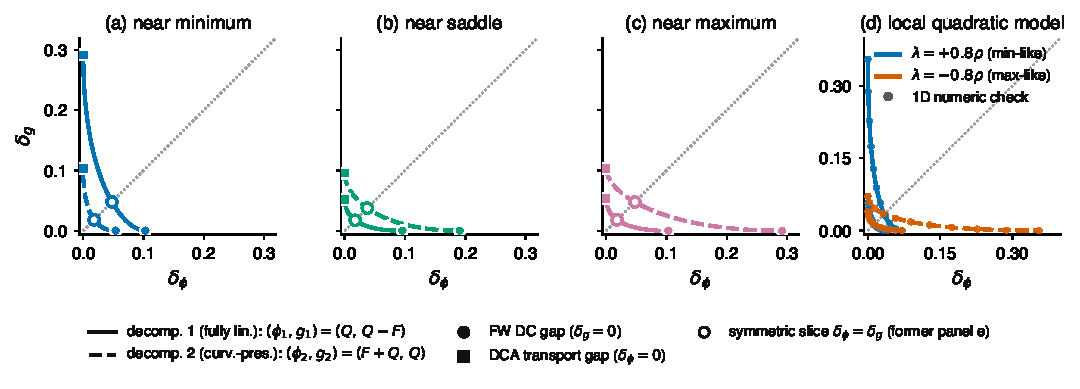
\includegraphics[width=\textwidth]{pareto_frontier_decomposition.pdf}
    \caption{Decomposition dependence read on the $(\delta_\phi,\delta_g)$
    scale, on the example of \citet[Figure~1]{maskan2025}:
    $F(\bx)=\sin(\pi x_1)\cos(\pi x_2)$, $L=\pi^2$, with
    $Q=\frac{L}{2}\|\cdot\|^2$ and the two convex decompositions
    $(\phi_1,g_1)=(Q,\,Q-F)$ (fully linearized, solid) and
    $(\phi_2,g_2)=(F+Q,\,Q)$ (curvature preserving, dashed). A certificate
    $\bv$ lies in $\partial_\delta h(\bar\bx)$ exactly when its Fenchel gap
    $h(\bar\bx)+h^{*}(\bv)-\langle\bv,\bar\bx\rangle\le\delta$; each curve is
    the lower-left (Pareto) boundary of the slack pairs
    $(\delta_\phi,\delta_g)$ for which a \emph{single} certificate $\bv$
    renders $\bar\bx$ a $(\delta_\phi,\delta_g,0)$-critical point of
    $(\phi_i,g_i)$.
    \textbf{a}--\textbf{c}: frontiers at three probe points
    $\bar\bx=\bx^{*}+d\,\bu$ ($d=0.15$, $\bu$ the leading Hessian eigenvector
    of $F$ at the stationary point $\bx^{*}$) near the global minimum, a
    saddle, and the global maximum. On each curve the $\delta_g=0$ intercept
    ($\bullet$) is the Frank--Wolfe DC gap of that decomposition
    (\Cref{lem:gap-dc-slice}), the $\delta_\phi=0$ intercept ($\blacksquare$)
    is the DCA transport gap, and the diagonal $\delta_\phi=\delta_g$ section
    ($\circ$) recovers the symmetric single-dial reading of the mismatch
    $\eps^{*}_{\delta}$. The two decompositions trace genuinely different
    frontiers, and their $\delta_g=0$ intercepts swap order between the
    minimum (curvature preserving smaller) and the maximum (fully linearized
    smaller): the qualitative effect reported by \citet{maskan2025}, localized
    here to an intercept property. Every frontier contracts to the origin as
    $\bar\bx\to\bx^{*}$ at rate $O(d^2)$.
    \textbf{d}: local quadratic model. Along an eigendirection of curvature
    $\lambda$, writing $\rho=L$, the frontiers are
    $\sqrt{2(\rho+\lambda)\delta_\phi}+\sqrt{2\rho\,\delta_g}=|\lambda d|$
    (curvature preserving) and
    $\sqrt{2\rho\,\delta_\phi}+\sqrt{2(\rho-\lambda)\delta_g}=|\lambda d|$
    (fully linearized): moving $F$ across the decomposition transfers the
    curvature coefficient from the $\delta_\phi$ scale to the $\delta_g$
    scale. Dots: matching one-dimensional numeric frontiers on
    $F(t)=\frac{\lambda}{2}t^{2}$. Conjugates of the nonquadratic components
    are evaluated on a grid.}
    \label{fig:decomposition-dependence}
\end{figure}

\Cref{fig:decomposition-dependence} reads the same example on the
$(\delta_\phi,\delta_g)$ scale. At every probe point the two
decompositions trace different Pareto frontiers, yet each is pinned by
the same landmarks: its $\delta_g=0$ intercept is the decomposition's
Frank--Wolfe DC gap and its $\delta_\phi=\delta_g$ section is the
symmetric mismatch reading. The Frank--Wolfe intercepts reproduce the
observation of \citet{maskan2025}---curvature preserving is cheaper near
the minimum and dearer near the maximum---while the whole frontier
shrinks to the origin as $\bar\bx$ approaches the stationary point,
uniformly in the decomposition, in line with
\Cref{prop:vanishing-decomposition-dependence}. In summary, the
trade-off identified by \citet{maskan2025} is real but lives on the
achievability side, namely which certificates a given decomposition
renders cheap to compute. The certificates themselves, expressed in the
$(\delta_\phi,\delta_g,\eps)$ coordinates, subsume the Frank--Wolfe gap
as a $(\delta,0,0)$-slice (\Cref{lem:gap-dc-slice}), transfer without
loss under convex shifts (\Cref{lem:convex-shift-transfer}), and
degrade in a controlled $O(\sqrt{\lambda\delta})$ fashion between
smooth decompositions
(\Cref{prop:vanishing-decomposition-dependence}).

